\documentclass[11pt,letterpaper]{article}
\usepackage[margin=1in]{geometry}
\usepackage[T1]{fontenc}
\usepackage{times}
\renewcommand{\ttdefault}{cmtt}
\usepackage[super,comma,sort&compress]{natbib}
\usepackage{graphicx}
\usepackage{booktabs}
\usepackage{amsmath}
\usepackage{caption}
\usepackage{xcolor}
\usepackage[hidelinks]{hyperref}
\captionsetup{font=small,labelfont=bf,labelsep=period}
\setlength{\parskip}{0.35em}
\renewcommand{\bibnumfmt}[1]{#1.}

\title{\bfseries Accept or abstain? A pre-specified test of reliability gates calibrated on held-out chemistry for molecular property and reaction-yield models}
\author{Oleksandr Gurbych\\[0.3em]
\small Blackthorn AI Ltd., London, United Kingdom\\
\small ORCID 0000-0002-6821-3390 \quad Correspondence: alex@blackthorn.ai}
\date{Working revision: 12 November 2026 (not posted)}

\begin{document}
\maketitle

\begin{abstract}
\noindent A molecular property or reaction-yield model is useful to a chemist only when it is right on the query in front of them, yet a model's uncertainty is rarely checked on chemistry it has not seen. We tested an accept-or-abstain protocol in which a gate, scoring each query by its similarity to the training set and by ensemble spread, returns a prediction only when it accepts the query. The gate uses an empirical binomial-test threshold rule inspired by Learn-then-Test, with a target precision on a calibration fold held out by chemistry rather than at random; no finite-sample guarantee is established for this implementation. On public data (23,401 logP values from SangsterLogP with two overlapping external sets, and the Buchwald--Hartwig and Suzuki--Miyaura high-throughput yield datasets), we evaluated eight held-out tests against four hypotheses defined in advance. Ranking queries by the gate's score lowered the error rate at 30\% coverage by 0.16 to 0.35 on seven of the eight tests. At a target precision of 0.8, the complete calibration pipelines differed most for yields: gates calibrated on a random fold accepted almost every reaction with an unseen additive at a precision of 0.59 to 0.75, whereas gates calibrated on held-out additives reached a pooled precision of 0.85 to 0.87 on three of the four tests, at lower coverage. At a target of 0.9, random-fold gates came within 0.05 of the target on three of the four tests. For the random forest, fusing similarity with spread did no better than spread alone, and conformal intervals calibrated on a random fold lost coverage under shift (down to 0.64). On a fluorinated-compound hold-out, the fused score showed no clear error reduction at 30\% coverage, and the held-out-calibrated gate missed its target. All four hypotheses therefore failed their complete success criteria for the primary model. In an exploratory analysis, intervals calibrated on the held-out fold reached empirical coverage of at least 0.90 on seven of the eight tests, at the cost of greater width; this does not establish conformal validity under shift. A graph network added by a protocol amendment before it was run, an ensemble of five directed message-passing networks, was the most accurate learner on logP and the least accurate on yields; with it, as with the random forest, ensemble spread ranked errors better than similarity on seven of the eight tests, fusion again improved on the better signal by less than 10\%, and all four hypotheses again failed. We release the protocol, the code and the complete results.
\end{abstract}

\noindent\textbf{Keywords:} applicability domain, selective prediction, conformal prediction, uncertainty quantification, lipophilicity, reaction yield

\section{Introduction}

Machine-learning models are now routine in medicinal chemistry and synthesis planning. They estimate lipophilicity, solubility and toxicity before a compound is made, and they score reaction conditions before a plate is run. A chemist uses such a prediction one compound or one reaction at a time. What matters to them is therefore not the average error over a benchmark, but whether this particular prediction can be trusted.

The usual way of reporting accuracy does not answer that question. Most models are evaluated on a random split of one dataset, so the test molecules resemble the training molecules closely. It is well documented that random splits overstate performance on new chemistry, and that scaffold, cluster and time splits give a more sober picture.\cite{sheridan2013,wallach2018,yang2019} Our own earlier work met the same problem in three settings. A graph network for chemical yields, comparable with the best published models on random splits, lost much of its accuracy on Buchwald--Hartwig reactions with unseen additives.\cite{yarish2023} A binding-affinity graph network that reached an $R^2$ of 0.50 on random splits fell to 0.11 on the hardest of its held-out splits.\cite{nikolaienko2022} Published logP models, including the Crippen atom-contribution method\cite{wildman1999} and pre-trained graph networks, were inapplicable to saturated fluorine-containing compounds, while models trained on the new measurements were not.\cite{gurbych2025}

The idea that a model should be used only inside its applicability domain is as old as the OECD principles for QSAR validation.\cite{oecd2007} Regulators now ask a similar question of AI models in general: in its 2025 draft guidance the U.S. Food and Drug Administration frames model credibility in terms of a stated context of use.\cite{fda2025} In practice, however, few published molecular models state where they may be used, and fewer still check that statement on held-out chemistry.

A practical answer is to let the model abstain. If a model returns a prediction only when it is likely to be right, and says ``do not know'' otherwise, the precision of the predictions it does return may improve at the cost of coverage; whether it reaches a target must be checked. Two kinds of signal are commonly used to decide: the distance of the query from the training data, and the model's own uncertainty. Both are established, and neither dominates in published benchmarks.\cite{hirschfeld2020,scalia2020} What is less often tested is how the decision threshold is chosen. A threshold calibrated on a random fold is calibrated on queries that look like the training set, and there is no reason to expect it to hold on chemistry that does not.

This work tested that question directly. We built an accept-or-abstain gate from a similarity signal and an ensemble-spread signal, set its threshold with an empirical binomial-test rule to a stated target precision, and compared two complete pipelines using random or chemistry-held-out calibration folds. Switching folds also refits the fused scorer; the comparison does not isolate threshold calibration. We set four hypotheses, with success criteria, before the evaluation: that the gate lowers the error rate on held-out chemistry (H1); that random-fold calibration misses its target there while held-out-fold calibration meets it (H2); that combining the two signals ranks errors better than either alone (H3); and that gating restores the coverage of conformal intervals lost under shift (H4).

Hence, our contribution is fourfold:
\begin{enumerate}
\item We describe a six-step accept-or-abstain protocol for molecular models and release a reference implementation under the MIT licence.
\item We evaluated it on public lipophilicity and reaction-yield data against eight held-out tests, including the four published out-of-sample additive tests of the Buchwald--Hartwig dataset and a fluorinated-compound hold-out built from our measured logP data.
\item We report the outcome of all four hypotheses, including those that failed, together with an operating-limits card for each held-out test.
\item By a protocol amendment fixed before it was run, we repeated the evaluation with a graph network and compared, across three learners, which signal ranks errors best.
\end{enumerate}

\subsection{Related works}

The applicability-domain literature in QSAR is extensive. Sheridan et al.\ showed that the similarity of a query to its nearest training molecules is a good discriminator of prediction accuracy.\cite{sheridan2004} Tetko et al.\ compared distance-to-model measures on environmental-toxicity models and found that the spread of an ensemble of models was among the most reliable.\cite{tetko2008} Kaneko and Funatsu likewise defined an applicability domain from ensemble disagreement.\cite{kaneko2014} Tropsha's review of best practices made the applicability domain a required part of model reporting.\cite{tropsha2010}

Ordinary split-conformal prediction gives intervals with guaranteed marginal coverage when the fitted scoring rule is fixed independently of calibration observations and calibration and test scores are exchangeable.\cite{vovk2005,lei2018} Norinder et al.\ introduced it to QSAR as an alternative to applicability-domain rules.\cite{norinder2014} The guarantee need not survive a distribution shift; Tibshirani et al.\ showed how to repair it when the likelihood ratio of the shift is known,\cite{tibshirani2019} which in chemistry it rarely is. Morger et al.\ showed on time-split bioactivity data and on toxicity endpoints that updating the calibration set with data more similar to the test set often improved empirical prediction-set coverage for conformal classifiers under data drift, at a cost in efficiency.\cite{morger2022}

Selective prediction treats abstention as part of the model. Geifman and El-Yaniv analysed the risk--coverage trade-off of selective classifiers.\cite{geifman2017} Learn-then-Test by Angelopoulos et al.\ turns the choice of an abstention threshold into a multiple-testing problem, which can yield risk control under its stated sampling and multiple-testing assumptions, including independent and identically distributed calibration observations.\cite{angelopoulos2021} For molecular property prediction, Hirschfeld et al.\ and Scalia et al.\ benchmarked uncertainty estimates for graph networks, including deep ensembles,\cite{lakshminarayanan2017} and found that their ranking of errors depends on the dataset and on the split.\cite{hirschfeld2020,scalia2020}

On reaction yields, the Buchwald--Hartwig dataset of Ahneman et al.\ came with four out-of-sample tests on additives unseen in training.\cite{ahneman2018} Chuang and Keiser showed that much of the reported accuracy could be obtained from features without chemical meaning.\cite{chuang2018} Schwaller et al.\ reported strong random-split results with a transformer and weaker results on the out-of-sample tests,\cite{schwaller2021} as did our directed message-passing network.\cite{yarish2023} The Suzuki--Miyaura dataset of Perera et al.\ has been used mostly with random splits.\cite{perera2018}

\subsection{Objective of the study}

The primary objective of this work was to find out whether a reliability gate, calibrated in a way a practitioner can reproduce, achieves its empirical precision target on chemistry the model has not seen. For this purpose we deliberately used simple, widely available ingredients: fingerprints, a random forest, a small neural ensemble, nearest-neighbour similarity and a binomial test; a later, pre-specified amendment added a graph network. If the gate works with these, it can be added to most existing models; if it does not, the reasons are easier to see.

\section{Data}

\subsection{Lipophilicity}

The logP pool is the SangsterLogP dataset of Cirino et al.,\cite{cirino2026,sangsterzenodo} which contains 23,520 curated measurements. After parsing with RDKit,\cite{rdkit} removal of duplicates by InChIKey, and removal of every compound that occurs in either external set, 23,401 compounds remained. Two external sets were held out completely. E1 is the prospective set distributed with SangsterLogP (327 compounds); 182 of them are the amides measured for our 2025 study.\cite{gurbych2025} E2 is the set of 183 amide logP values from that study, as released in its public repository. In E2, 140 compounds contain an sp\textsuperscript{3} carbon--fluorine bond (SMARTS \texttt{[CX4]F}), and 43 are their non-fluorinated parents or methyl analogues.

\subsection{Reaction yields}

The Buchwald--Hartwig (BH) dataset of Ahneman et al.\ contains 3,955 Pd-catalysed C--N couplings of aryl halides with \textit{p}-toluidine, varying the aryl halide, ligand, base and an isoxazole additive.\cite{ahneman2018} We used the four published out-of-sample tests, in which five of the 22 additives appear only in the test rows. The Suzuki--Miyaura (SM) dataset of Perera et al.\ contains 5,760 couplings varying both coupling partners, the ligand (eleven ligands and a ligand-free control), the base and the solvent; we used the UV-area yield.\cite{perera2018} Both datasets were taken from the public redistribution that accompanied our earlier yield study.\cite{yarish2023} For SM, each component name was mapped to its structure using a table written for this study, with spectator fragments such as the internal standard omitted.

It is worth mentioning that both reaction datasets come from single high-throughput campaigns. Their chemistry is narrow, and a large share of reactions gave little or no product. A ``held-out'' additive or ligand is therefore a small, controlled shift, and not new chemistry in the sense a medicinal chemist would use. We return to this point in Section~\ref{sec:limits}.

\section{Methodology}

\begin{figure}[t]
\centering
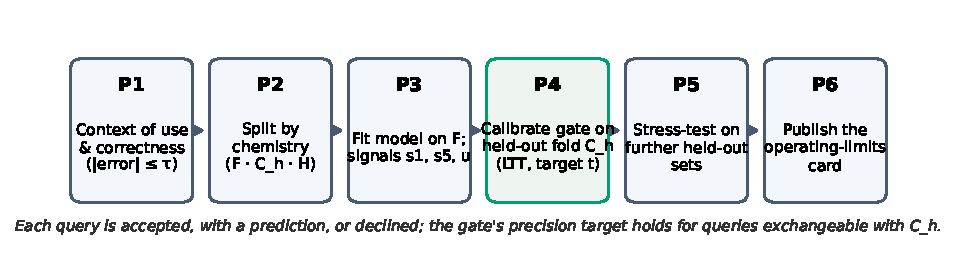
\includegraphics[width=\linewidth]{figures/fig1_protocol.pdf}
\caption{The accept-or-abstain protocol. P1: state the context of use and what counts as a correct prediction. P2: split the data by chemistry into a fit set $F$, a held-out calibration fold $C_h$ and held-out tests. P3: fit the model and compute the signals. P4: calibrate the gate on $C_h$ to a target precision. P5: test it on further held-out sets. P6: publish the operating limits.}
\label{fig:protocol}
\end{figure}

\subsection{Protocol}

The protocol has six steps (Figure~\ref{fig:protocol}). The user first states what a correct prediction is for the intended use (P1). In this study a logP prediction was correct if its absolute error was at most 0.5 log units, and a yield prediction if its absolute error was at most 10 percentage points. Coverage is the share of queries the gate accepts; selective precision is the share of accepted queries that are correct; the selective error rate is one minus selective precision. The data are then split by chemistry (P2), the model and its signals are fitted (P3), the gate is calibrated on a fold held out by chemistry to a target precision $t$ (P4), it is tested on further held-out sets (P5), and the result is published as an operating-limits card (P6): for each target and test, the coverage and the precision actually achieved.

The hypotheses and their success criteria (Section~\ref{sec:hypotheses}) were set before the evaluation; the full analysis plan is given in the Supporting Information. Analyses outside the plan are marked as exploratory.

\subsection{Representations and models}

Molecules were represented by ECFP4 count vectors\cite{rogers2010} (radius 2, 2,048 bins) together with ten RDKit descriptors (molecular weight, TPSA, numbers of H-bond donors and acceptors, rotatable bonds, rings, aromatic rings, heavy atoms and heteroatoms, and the fraction of sp\textsuperscript{3} carbons). The Crippen logP descriptor was deliberately excluded, so that the model could not simply correct a known estimator. Reactions were represented by concatenating 1,024-bit ECFP4 vectors of each variable component.

The primary model (M1) was a random forest\cite{breiman2001} of 300 trees with 20\% of features considered at each split; its spread $u$ is the standard deviation of the per-tree predictions. The secondary model (M2), used only to check robustness, was an ensemble of five multilayer perceptrons (512 and 128 hidden units, ReLU, Adam, L2 penalty $10^{-4}$, early stopping on 10\% of the fit set); its spread is the standard deviation across members.\cite{lakshminarayanan2017} Both were implemented in scikit-learn.\cite{pedregosa2011} Hyper-parameters were set in advance and not tuned.

A third learner (M3) was added after the first version had been scored, by a protocol amendment (2.0) fixed before any M3 prediction was computed (Supporting Information, Section~S3). With M1 the fused score had ranked errors no better than spread, whereas with M2 similarity had ranked logP errors better than spread, so the outcome of H3 might depend on the learner. M3 is an ensemble of five directed message-passing neural networks (D-MPNN),\cite{yang2019} trained with Chemprop 2.3.1\cite{heid2024chemprop} at its default settings, which were not tuned: bond-based message passing with hidden size 300 and depth 3, norm aggregation, one hidden feed-forward layer of 300 units, a mean-squared-error loss on standardised targets, batch size 64 and 50 epochs, with a random 10\% of the fit set selecting the checkpoint. A compound enters as its SMILES; a reaction enters as the SMILES of its components joined into one multi-fragment graph. Its spread $u$ is the standard deviation across members. The similarity signals, gates and metrics are computed exactly as for M1 and M2, and H1--H4 are applied to M3 with unchanged criteria.

\subsection{Splits}

\begin{table}[t]
\centering
\caption{Datasets and splits. Sizes are means over five seeds. $F$: fit set; $C_r$: random calibration fold; $C_h$: held-out calibration fold; $R$: random (in-distribution) test; $H$: held-out test.}
\label{tab:splits}
\resizebox{\linewidth}{!}{\begin{tabular}{@{}llrrrrrl@{}}
\toprule
Task & Groups (number) & $F$ & $C_r$ & $C_h$ & $R$ & $H$ & Held-out tests \\
\midrule
LogP (D1) & Butina cluster (3,349) & 11,429 & 2,449 & 3,522 & 2,449 & 3,551 & cluster; E1 (327) \\
LogP, no sp\textsuperscript{3} C--F (D1) & Butina cluster (3,160) & 10,656 & 2,283 & 3,327 & 2,284 & 3,308 & cluster; E2 (183) \\
Buchwald--Hartwig Test1--4 (D3a) & additive (17 + 5) & 1,636 & 351 & 719 & 350 & 898 & 5 unseen additives \\
Suzuki--Miyaura (D3b) & ligand (12) & 2,688 & 576 & 960 & 576 & 960 & 2 unseen ligands \\
\bottomrule
\end{tabular}}
\end{table}

For each task the pool was divided by a group label: Butina clusters\cite{butina1999} of ECFP4 at a Tanimoto distance of 0.65 for logP (3,349 clusters), the additive for BH, and the ligand for SM. Whole groups were assigned to a held-out test $H$, to a held-out calibration fold $C_h$, and to an in-distribution part. For logP, $H$ and $C_h$ each received about 15\% of the compounds. For BH, $H$ was the published test of each TestN, and four of the 17 training additives formed $C_h$. For SM, two ligands formed $H$ and two others $C_h$; the ligand-free control counted as one of the twelve ligands and could be drawn for either role. The in-distribution part was split at random into the fit set $F$ (70\%), a random calibration fold $C_r$ (15\%) and a random test $R$ (15\%). Every model was trained on $F$ alone, and both gates used the same model. Table~\ref{tab:splits} gives the sizes.

Holding out calibration additives leaves about 1,640 BH reactions in $F$, roughly half of the published training rows, so ungated BH accuracy is not directly comparable with published results on the same tests. To build the fluorinated hold-out, a separate logP model was trained after removing all 1,543 compounds with an sp\textsuperscript{3} C--F bond from the pool, and was scored on E2. Five seeds (0--4) were used throughout.

\subsection{Signals}

Two signals of input novelty were computed against $F$: $s_1$, the largest Tanimoto similarity of the query fingerprint to any compound or reaction in $F$, and $s_5$, the mean of the five largest. The confidence signal was the ensemble spread $u$. For intervals with nominal 90\% coverage, we used a normalised conformal-style rule inspired by split-conformal prediction\cite{lei2018} with the score $|y-\hat{y}|/(u+\varepsilon)$, where $\varepsilon$ is 0.1 times the median spread on the calibration fold. For $n$ calibration scores, the implementation takes NumPy's ``higher'' quantile at $\min(1,\lceil(n+1)0.9\rceil/n)$ and returns $\hat{y}\pm q(u+\varepsilon)$. This quantile convention need not equal the usual $\lceil(n+1)0.9\rceil$-th order statistic. We retain it to reproduce the original results. Because the normalizer uses calibration observations, we have not established the independence and exchangeability conditions for ordinary split-conformal coverage for this implementation. Distribution shift further undermines those conditions, and selection by a gate does not automatically preserve marginal coverage on the accepted subset. All reported interval coverages are empirical.

\subsection{Gates}

Every calibration fold was split at random into halves $C_a$ and $C_b$. Switching from $C_r$ to $C_h$ changes the scorer-fitting data, the threshold-selection data and generally their sizes; only the base model trained on $F$ stays fixed. Gate~B, the fused gate, is a logistic regression of correctness on $(s_1, s_5, \log(u+10^{-6}))$, fitted on $C_a$; its score is the predicted probability that the prediction is correct. For comparison, the single-signal gates use $s_1$ or $-u$ directly as the score.

Thresholds were selected on $C_b$ by an empirical binomial-test sequence inspired by Learn-then-Test.\cite{angelopoulos2021} Candidate thresholds are the score values in $C_b$, tested in a fixed sequence from the strictest one that accepts at least 50 points to looser ones. A threshold that accepts $n$ points of $C_b$, $k$ of them correct, passes if
\begin{equation}
p = \Pr\left[\mathrm{Bin}(n, t) \ge k\right] \le \delta, \qquad \delta = 0.1,
\end{equation}
and the loosest threshold reached before the first failure is used. If no threshold passes, the gate abstains on every query. Because the candidate thresholds and their sequence depend on the calibration data used for testing, and the external tests involve distribution shifts, we do not establish a finite-sample selective-precision guarantee for this implementation. Here $\delta$ is the per-candidate test cutoff, not a proved probability of attaining the target on future queries. We report achieved precision and acceptance coverage empirically. The historical code name \texttt{ltt\_threshold} and result labels \texttt{LTT\_*} identify this implemented rule, not a certified Learn-then-Test procedure. Gate~A, a conjunctive empirical baseline, accepts a query if $s_1 \ge \tau_1$ and $u \le \tau_2$, with the pair chosen from a $20\times20$ grid of quantiles on the whole calibration fold as the largest coverage whose empirical precision is at least $t$. Targets were $t = 0.8$ and $0.9$.

\subsection{Metrics and hypotheses}
\label{sec:hypotheses}

For each test we report RMSE, MAE and $R^2$ without a gate; the risk--coverage curve of each score, that is, the selective error rate when the $k$ highest-scoring queries are accepted; the area under that curve (AURC); the coverage and achieved precision of each gate; and the empirical coverage of the conformal intervals. Results are averaged over seeds. Bootstrap intervals resample test queries; for test sets that are identical in every seed (E1, E2 and BH Test1--Test4), the same resample is used for all seeds. The held-out tests are the logP cluster test, E1 and E2 (the D1 family), and BH Test1--Test4 and the SM ligand test (the D3 family). E1 and E2 share 182 compounds and are therefore not independent tests. The BH tests share a campaign and training data; the eight tests are not eight independent replications. Results are reported by test and family.

The operating-limits cards report descriptive precision pooled over accepted prediction--seed observations, with exact correct/accepted counts. The same query may occur in several seeds; these observations are not independent binomial trials. We therefore remove the original pooled Wilson intervals rather than substitute another interval without a justified sampling target. Per-seed precision, counts and coverage for both pipelines are provided in Tables S5--S8 and machine-readable files. No interval for a population of new chemical groups or campaigns is claimed. The original H1 query-bootstrap intervals are retained to evaluate the original criterion conditional on the fitted pipelines; for logP $H$ and SM $H$, whose held-out sets differ by seed, queries are resampled separately within each seed even when those sets partly overlap. Those intervals therefore do not preserve all repeated-query dependence, chemical-group dependence or training-set uncertainty, and should not be read as evidence for new-campaign generalization. An inferential extension would need paired resampling of repeated queries together with justified chemical/reaction clusters and a defined population target. The hypotheses, decided on M1, were:
\begin{description}
\item[H1] On every held-out test, the fused score's selective error rate at 30\% coverage is below the ungated error rate, with a 95\% bootstrap interval of the difference that excludes zero.
\item[H2] Over the 16 (test $\times$ target) cells, Gate~B calibrated on $C_r$ misses its target by more than 0.05 in at least half; calibrated on $C_h$, it reaches at least $t-0.05$ in at least three quarters.
\item[H3] Gate~B's AURC is at least 10\% lower than that of the better single signal on at least two held-out tests in each family.
\item[H4] Conformal intervals calibrated on $C_r$ cover at least 0.88 of $R$, fall below 0.85 on at least one held-out test, and recover to at least 0.88 on the queries accepted by Gate~B ($C_h$, $t=0.8$) wherever they fell.
\end{description}

\section{Results and discussion}

\subsection{The accuracy gap}

\begin{figure}[t]
\centering
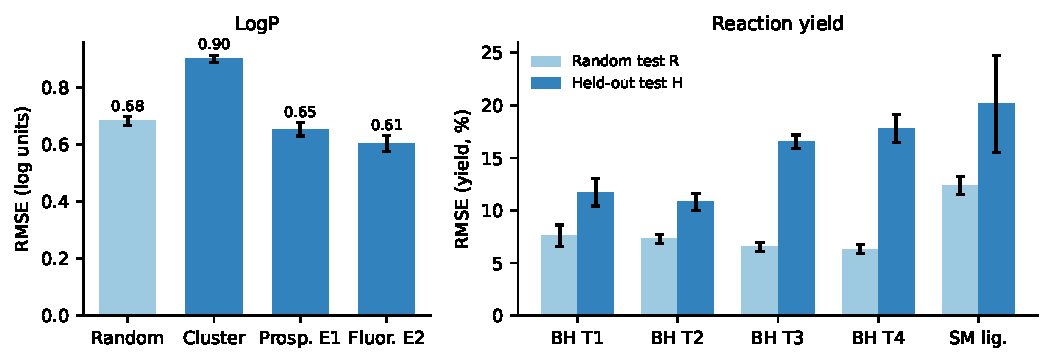
\includegraphics[width=\linewidth]{figures/fig2_gap.pdf}
\caption{Ungated RMSE of M1 on the random test $R$ and on the held-out tests (mean $\pm$ s.d. over five seeds). Left: logP. Right: reaction yields.}
\label{fig:gap}
\end{figure}

\begin{table}[t]
\centering
\caption{Ungated accuracy of M1 (mean $\pm$ s.d. over five seeds). Error rate: share of predictions with an absolute error above 0.5 log units (logP) or 10 percentage points (yield).}
\label{tab:accuracy}
\small
\begin{tabular}{@{}lrrrr@{}}
\toprule
Test set & $n$ & RMSE & $R^2$ & Error rate \\
\midrule
LogP, random $R$ & 2,449 & 0.68 $\pm$ 0.02 & 0.84 $\pm$ 0.01 & 0.37 \\
LogP, held-out cluster & 3,551 & 0.90 $\pm$ 0.01 & 0.70 $\pm$ 0.02 & 0.49 \\
LogP, prospective E1 & 327 & 0.65 $\pm$ 0.02 & 0.58 $\pm$ 0.03 & 0.38 \\
LogP, fluorinated E2 (all) & 183 & 0.61 $\pm$ 0.03 & -0.07 $\pm$ 0.10 & 0.36 \\
\quad sp\textsuperscript{3} C--F compounds & 140 & 0.60 $\pm$ 0.03 & -0.25 $\pm$ 0.13 & 0.34 \\
\quad parents & 43 & 0.63 $\pm$ 0.02 & 0.23 $\pm$ 0.04 & 0.40 \\
\addlinespace
BH Test1, random $R$ & 350 & 7.60 $\pm$ 1.02 & 0.92 $\pm$ 0.02 & 0.14 \\
BH Test1, held-out additives & 898 & 11.71 $\pm$ 1.29 & 0.81 $\pm$ 0.04 & 0.28 \\
BH Test2, random $R$ & 351 & 7.30 $\pm$ 0.45 & 0.93 $\pm$ 0.01 & 0.15 \\
BH Test2, held-out additives & 900 & 10.81 $\pm$ 0.82 & 0.84 $\pm$ 0.02 & 0.27 \\
BH Test3, random $R$ & 350 & 6.54 $\pm$ 0.42 & 0.94 $\pm$ 0.01 & 0.12 \\
BH Test3, held-out additives & 897 & 16.54 $\pm$ 0.63 & 0.65 $\pm$ 0.03 & 0.37 \\
BH Test4, random $R$ & 350 & 6.32 $\pm$ 0.45 & 0.95 $\pm$ 0.01 & 0.09 \\
BH Test4, held-out additives & 900 & 17.79 $\pm$ 1.35 & 0.55 $\pm$ 0.07 & 0.41 \\
\addlinespace
SM, random $R$ & 576 & 12.36 $\pm$ 0.87 & 0.81 $\pm$ 0.03 & 0.32 \\
SM, held-out ligands & 960 & 20.13 $\pm$ 4.63 & 0.23 $\pm$ 0.65 & 0.49 \\
\bottomrule
\end{tabular}
\end{table}

Most held-out tests were harder than the random test of the same task (Figure~\ref{fig:gap}, Table~\ref{tab:accuracy}); the two external logP sets were the exceptions. For logP, the RMSE rose from 0.68 on $R$ to 0.90 on held-out clusters, and the share of predictions outside 0.5 log units rose from 0.37 to 0.49. On E1 the RMSE was slightly lower than on $R$ (0.65 against 0.68), although the error rate was slightly higher (0.38 against 0.37). For the BH additive tests the RMSE rose 1.5- to 2.8-fold, from 6.3--7.6 to 10.8--17.8 percentage points, with $R^2$ of 0.81, 0.84, 0.65 and 0.55 on Test1--Test4. For SM, holding out two ligands raised the RMSE from 12.4 to 20.1, and $R^2$ varied from $-0.90$ to $0.73$ across seeds (mean 0.23), depending on which ligands were held out. The lowest value came from seed 0, in which the held-out pair was Xantphos and the ligand-free control.

The fluorinated hold-out behaved differently. The model trained without any sp\textsuperscript{3} C--F compound had a lower error rate on E2 (0.36) than on its own random test (0.37), and a lower RMSE (0.61 against 0.70). On the fluorinated compounds its error rate (0.34) was lower than on their parents (0.40). This does not show that the model had learned the effect of fluorination. Its $R^2$ on the sp\textsuperscript{3} C--F compounds was $-0.25$, indicating greater squared error than the test-set mean reference, not absence of rank association, and the logP values in E2 span a narrow range: their standard deviation (0.59) is close to the 0.5 tolerance, and predicting the E2 mean for every compound would give an error rate of 0.40. That reference uses the test labels and is descriptive, not a deployable predictor. The low error rate on E2 therefore reflects the narrow range of the set more than predictive skill, and the problem that motivated our earlier study of these compounds\cite{gurbych2025} is not solved by this model.

\subsection{Which signal ranks errors}

\begin{figure}[t]
\centering
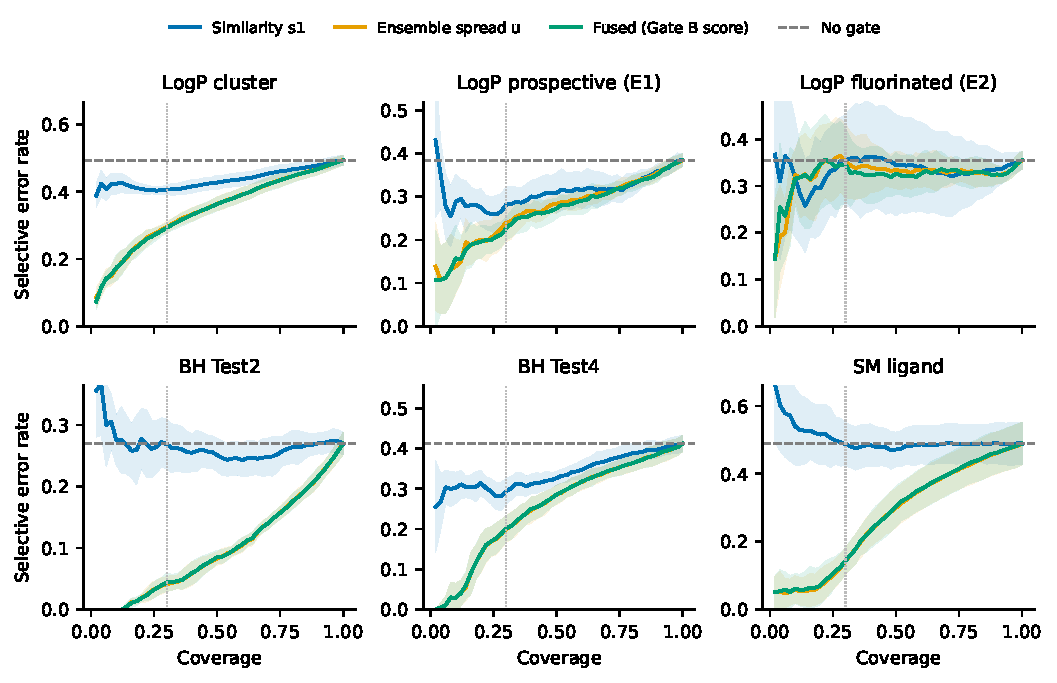
\includegraphics[width=\linewidth]{figures/fig3_risk_coverage.pdf}
\caption{Risk--coverage curves of M1 on six held-out tests (mean $\pm$ s.d. over seeds): selective error rate when the queries with the highest score are accepted. The fused score is fitted on $C_h$. The dashed line is the ungated error rate; the dotted line marks 30\% coverage (H1). BH Test1 and Test3, not shown, behave like Test2 (Table~\ref{tab:aurc}).}
\label{fig:rc}
\end{figure}

\begin{table}[t]
\centering
\caption{AURC of the selective error rate for M1 (lower is better; mean over seeds). ``No gate'' is the ungated error rate, i.e., the AURC of a random ordering.}
\label{tab:aurc}
\small
\begin{tabular}{@{}lrrrr@{}}
\toprule
Held-out test & No gate & $s_1$ & $-u$ & Fused \\
\midrule
LogP cluster & 0.494 & 0.436 & 0.343 & 0.342 \\
LogP prospective (E1) & 0.385 & 0.317 & 0.267 & 0.263 \\
LogP fluorinated (E2) & 0.355 & 0.337 & 0.323 & 0.322 \\
BH Test1 & 0.281 & 0.259 & 0.112 & 0.112 \\
BH Test2 & 0.270 & 0.267 & 0.097 & 0.097 \\
BH Test3 & 0.365 & 0.322 & 0.164 & 0.164 \\
BH Test4 & 0.412 & 0.337 & 0.251 & 0.251 \\
SM ligand & 0.489 & 0.503 & 0.271 & 0.273 \\
\bottomrule
\end{tabular}
\end{table}

Ranking queries by the fused score lowered the error rate on seven of the eight held-out tests (Figure~\ref{fig:rc}). At 30\% coverage, the error rate fell from 0.49 to 0.29 on held-out logP clusters, from 0.38 to 0.22 on E1, from 0.27--0.41 to 0.04--0.20 on the four BH tests, and from 0.49 to 0.14 on the SM ligand test; each original query-bootstrap 95\% interval excluded zero. This describes the original H1 criterion, with the dependence limitations stated in Section~\ref{sec:hypotheses}. On E2 it fell only from 0.355 to 0.345, with an interval of $-0.098$ to $+0.067$. Because H1 required every test, it does not hold, although its original computational criterion was met on seven of eight.

The ranking came almost entirely from the ensemble spread. For M1, the similarity signal $s_1$ was weaker than $-u$ on every held-out test (Table~\ref{tab:aurc}): only slightly on E2 (AURC 0.337 against 0.323), markedly on the others. On the reaction tests it was far weaker than the spread, and on the SM ligand test it was worse than a random ordering. This is partly built into the design. For reactions, $s_1$ is computed on the concatenated fingerprints of all components, and a reaction with a new additive or ligand still shares its other components with many reactions in $F$, so its similarity barely registers the change. A component-wise similarity would be a fairer test of H3 for reactions. The fused score therefore learned to follow $u$, and its AURC was within 2\% of that of $-u$ on every test, from 1.7\% better to 0.9\% worse. H3 does not hold for M1. This agrees with earlier reports that ensemble disagreement is one of the most reliable distance-to-model measures,\cite{tetko2008,kaneko2014} and with benchmarks in which no single uncertainty estimate dominated.\cite{hirschfeld2020,scalia2020}

In an exploratory check on E2, neither signal tracked the error: the rank correlation between absolute error and $u$ ranged from $-0.05$ to $0.22$ across seeds, compared with 0.28--0.38 on held-out clusters. The signals did register that the fluorinated compounds were unfamiliar: their mean $s_1$ was 0.43--0.46 across seeds, against 0.49--0.54 for the parents and 0.65--0.66 for the random test, and their spread was higher. But the model was not worse on them, so novelty and error were decoupled.

\subsection{Comparison of complete calibration pipelines}

\begin{figure}[t]
\centering
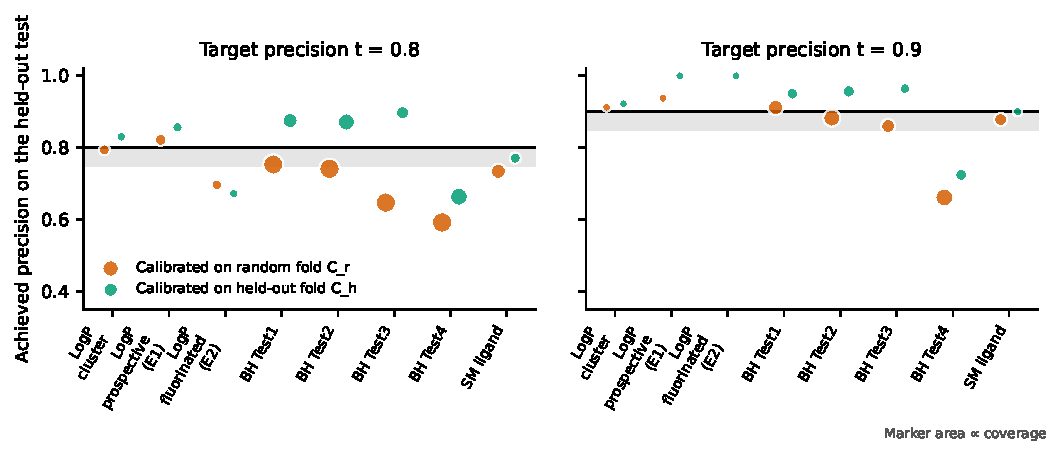
\includegraphics[width=\linewidth]{figures/fig4_calibration.pdf}
\caption{Precision achieved by Gate~B (M1) on each held-out test for the random-fold $C_r$ and held-out-fold $C_h$ pipelines (both scorer fitting and threshold selection change) (mean over seeds that accepted at least one query). The black line is the target; the grey band is the 0.05 tolerance of H2. Marker area is proportional to coverage.}
\label{fig:cal}
\end{figure}

\begin{table}[t]
\centering
\caption{Operating-limits card for Gate~B (M1) at target precision $t = 0.8$. Coverage is the mean over five seeds, including seeds that abstained on every query. Precision is a descriptive pooled estimate over accepted prediction--seed observations; correct/accepted counts and accepting seeds are shown for both pipelines. No independent-binomial interval is appropriate for these repeated predictions. Per-seed results are in Tables S5--S8. H2 is judged on seed-averaged precision (Figure~\ref{fig:cal}).}
\label{tab:card}
\small
\resizebox{\linewidth}{!}{\begin{tabular}{@{}lccccc@{}}
\toprule
 & \multicolumn{2}{c}{Calibrated on $C_r$} & \multicolumn{3}{c}{Calibrated on $C_h$} \\
\cmidrule(lr){2-3}\cmidrule(lr){4-6}
Held-out test & Coverage & Precision [95\% CI] & Coverage & Precision [95\% CI] & Seeds accepting \\
\midrule
LogP cluster & 0.13 & 0.79 [0.78, 0.81] & 0.05 & 0.82 [0.79, 0.84] & 3/5 \\
LogP prospective (E1) & 0.19 & 0.78 [0.73, 0.82] & 0.08 & 0.83 [0.75, 0.88] & 3/5 \\
LogP fluorinated (E2) & 0.12 & 0.72 [0.62, 0.79] & 0.04 & 0.71 [0.54, 0.83] & 3/5 \\
BH Test1 & 0.94 & 0.75 [0.74, 0.77] & 0.44 & 0.87 [0.86, 0.89] & 4/5 \\
BH Test2 & 0.98 & 0.74 [0.73, 0.75] & 0.62 & 0.85 [0.84, 0.86] & 5/5 \\
BH Test3 & 0.98 & 0.65 [0.63, 0.66] & 0.29 & 0.85 [0.83, 0.86] & 4/5 \\
BH Test4 & 0.99 & 0.59 [0.58, 0.61] & 0.70 & 0.64 [0.62, 0.65] & 5/5 \\
SM ligand & 0.45 & 0.73 [0.71, 0.75] & 0.14 & 0.74 [0.70, 0.77] & 2/5 \\
\bottomrule
\end{tabular}}
\end{table}

The complete pipelines differed most for reaction yields (Figure~\ref{fig:cal}, Table~\ref{tab:card}). On the BH additive tests, gates calibrated on $C_r$ accepted 94--99\% of reactions and reached a precision of only 0.59--0.75 against a target of 0.8. A random calibration fold contains reactions with additives seen in training; on those, the model is accurate and the threshold is loose. Gates calibrated on $C_h$, whose additives were also unseen, reached a pooled precision of 0.87, 0.85 and 0.85 on Test1--Test3 (seed-averaged 0.88, 0.87 and 0.90). They did so by accepting fewer reactions: 44\%, 62\% and 29\%. Test4 was the exception. There the $C_h$ gate reached only 0.64, at 70\% coverage. Test4 is also the hardest test without a gate (error rate 0.41), and the four calibration additives did not represent its observed difficulty adequately. On the SM ligand test the two folds gave similar pooled precision (0.73 for $C_r$, 0.74 for $C_h$), and the $C_h$ gate accepted queries in only two of the five seeds. At the stricter target of 0.9, the difference between the folds was smaller: $C_r$-calibrated gates reached a pooled 0.91, 0.87 and 0.85 on BH Test1--Test3, within 0.05 of the target, and only Test4 (0.65) fell well short (Table~S4).

For logP, both calibration folds gave similar precision on the held-out tests, and both gates were very conservative. On held-out clusters the $C_h$ gate accepted 5\% of compounds at a pooled precision of 0.82, and it abstained completely in two of the five seeds. A random fold was not over-optimistic here, possibly because the threshold that reaches the target is so strict that it selects compounds close to the training set in either case; we did not test this.

Counting cells, $C_r$-calibrated gates missed the target by more than 0.05 in 6 of the 16 cells, short of the 8 required, while $C_h$-calibrated gates met $t-0.05$ in 13 of 16, above the 12 required. H2 therefore does not hold as a whole: its second part holds and its first does not. The misses of the $C_r$ gate were all on reactions, apart from the 0.8 target on E2. The second part is borderline. Several of its cells rest on a single accepting seed with few compounds (E2 at $t = 0.9$: two compounds; E1 at $t = 0.9$: ten), and with pooled instead of seed-averaged precision it falls to 12 of 16, exactly at the threshold.

Two properties of the implemented rule help interpret these observations. First, the test is strict at the start of the sequence. With 50 accepted calibration points, it needs 45 correct to pass at $t = 0.8$ and 49 at $t = 0.9$; if the first eligible candidate fails, the gate abstains on everything. Ties can make that first candidate larger than 50. Second, target attainment is an empirical outcome here. In an exploratory count over single seeds, the $C_h$ pipeline met its target in 31 of the 45 seed-cells in which it accepted anything (69\%), and the $C_r$ pipeline in 15 of 67 (22\%). These dependent seed-cells are descriptive counts, not an estimate or test of a theoretical 90\% reliability guarantee.

The conjunctive Gate~A gave similar precision at somewhat higher coverage. On BH Test1, for example, both reached a seed-averaged precision of 0.88, Gate~A at 57\% coverage and Gate~B at 44\%; on the SM ligand test Gate~A accepted 26\% of reactions at 0.85, against 14\% at 0.77 for Gate~B. The procedures differ in their selection rule and in the data available for scorer fitting and threshold selection; this comparison does not isolate the cost of either choice.

\subsection{Conformal coverage under shift}

\begin{figure}[t]
\centering
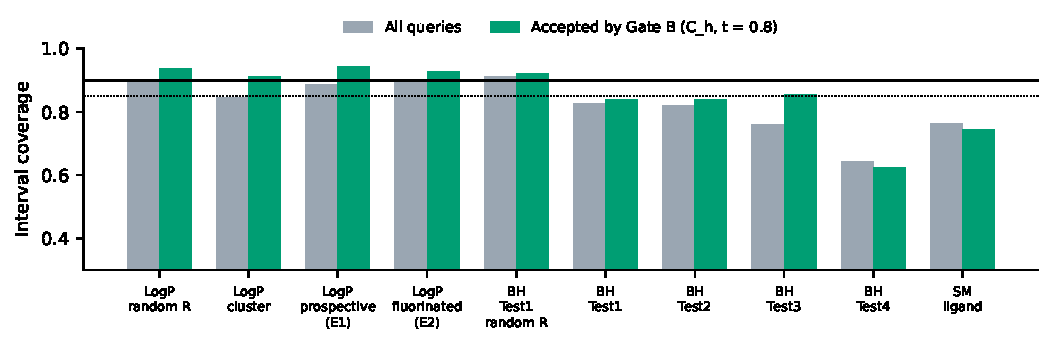
\includegraphics[width=\linewidth]{figures/fig5_conformal.pdf}
\caption{Empirical coverage of normalised conformal-style intervals (nominal 90\%, calibrated on $C_r$) for M1, on all queries and on the queries accepted by Gate~B ($C_h$, $t = 0.8$). Solid line: nominal level; dotted line: 0.85. Neither the full test nor the accepted subset has an established coverage guarantee for this implementation.}
\label{fig:conf}
\end{figure}

Calibrated on $C_r$, the nominal 90\% intervals empirically covered 0.88--0.92 of every random test (Figure~\ref{fig:conf}). Under shift they did not: coverage fell to 0.846 on held-out logP clusters, 0.83 and 0.82 on BH Test1 and Test2, 0.76 on Test3, 0.64 on Test4 and 0.76 on the SM ligand test. On logP clusters, the gate restored coverage to 0.91 on the accepted compounds. On the reaction tests it did not (0.62--0.85). A plausible reason is that the accepted reactions still carry the systematic offset of an unseen additive or ligand, which the ensemble spread does not see. H4 does not hold.

In an exploratory analysis we calibrated the same intervals on $C_h$ instead. They then covered at least 0.90 of the queries on seven of the eight held-out tests (0.90--0.96), and 0.80 on BH Test4, consistent with the empirical direction reported by Morger et al.\ under data drift.\cite{morger2022} Here changing folds changes both $\varepsilon$ and $q$, so this is a comparison of complete interval-calibration rules, not an isolated quantile-calibration effect or a proof of validity. The price is width: the intervals were about 1.2 times as wide as the $C_r$-calibrated ones for logP and 1.6--2.2 times for yields. On the SM ligand test they were 86 percentage points wide on average, too wide to be useful.

\subsection{The fluorinated case}

\begin{figure}[t]
\centering
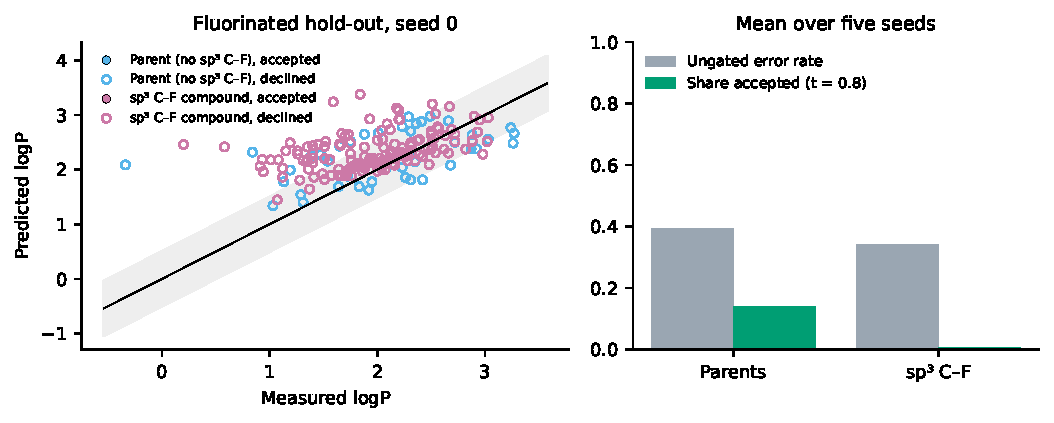
\includegraphics[width=\linewidth]{figures/fig6_fluorinated.pdf}
\caption{The fluorinated hold-out (M1 trained without sp\textsuperscript{3} C--F compounds). Left: predicted against measured logP for E2 in one seed; filled markers were accepted by Gate~B ($C_h$, $t = 0.8$); the grey band is $\pm 0.5$ log units. Right: ungated error rate and share accepted for parents and for sp\textsuperscript{3} C--F compounds, averaged over seeds.}
\label{fig:fl}
\end{figure}

Figure~\ref{fig:fl} shows the fluorinated case in detail. The gate declined almost every fluorinated compound: it accepted 0.6\% of them, against 14\% of the parents. Ungated precision on the fluorinated compounds was 0.66, already below the target of 0.8, so declining them was consistent with the target. But the compounds the gate did accept, mostly parents, had seed-averaged precision 0.67; the descriptive pooled precision was 0.71 (24 correct of 34 accepted prediction--seed observations; Table~\ref{tab:card}). The signals registered novelty (the fluorinated compounds had lower similarity and higher spread) without separating right from wrong predictions. Simpler gates did somewhat better on E2: the spread-only gate and Gate~A reached a seed-averaged precision of 0.77 and 0.78, at 4\% and 10\% coverage.

\subsection{Two further model families}

\begin{table}[t]
\centering
\caption{Hypotheses and their outcomes. M1 decides; M2 is a robustness check. M3 was added by protocol amendment 2.0 before any M3 prediction was computed; its verdicts do not change those of M1. For M2, H2 holds only vacuously: its $C_h$-calibrated gate abstained on every query of every held-out test, which counts as not missing the target.}
\label{tab:verdicts}
\small
\begin{tabular}{@{}llll@{}}
\toprule
Hypothesis & M1 (RF) & M2 (MLP) & M3 (D-MPNN) \\
\midrule
H1: gate lowers error at 30\% coverage & does not hold & holds & does not hold \\
H2: calibration split matters & does not hold & holds (vacuously) & does not hold \\
H3: fusion beats best single signal & does not hold & does not hold & does not hold \\
H4: gating restores conformal coverage & does not hold & does not hold & does not hold \\
\bottomrule
\end{tabular}
\end{table}

The MLP ensemble (M2) was somewhat more accurate than the random forest on random and held-out logP clusters (RMSE 0.62 and 0.84, against 0.68 and 0.90) and on the random BH tests, and similar on held-out additives (Table~S1, Supporting Information). It generalised worse to the fluorinated hold-out: its error rate on E2 was 0.48, against 0.36 for M1, and 0.50 on the sp\textsuperscript{3} C--F compounds alone. Its signals also behaved differently. On the logP tests, the similarity signal ranked errors better than the spread of the MLP ensemble, and the fused score improved on the better single signal by 7.4\%, 2.8\% and 5.7\% (Table~S2). That is more than for M1, but short of the 10\% that H3 requires. On reactions, the fused score was no better than spread, and on the SM test it was 7\% worse. H3 therefore fails for M2 too.

M2 met the original H1 computational criterion on all eight tests, although the reductions on reactions were small (0.03 to 0.09). The $C_h$-calibrated gate of M2, however, abstained on every query of every held-out test (Table~S3): on the held-out calibration folds, no threshold that accepted at least 50 points passed the binomial test (Section~4.3). On the BH Test1 calibration folds, for example, the 50 highest-scoring reactions had a precision of only 0.58--0.74. H2 therefore holds for M2 only vacuously, because a gate that accepts nothing counts as not missing its target, and H4 cannot be checked. The $C_r$-calibrated gate of M2 missed its target on every BH test by a wider margin than M1, with a precision of 0.52--0.70 at $t = 0.8$. Table~\ref{tab:verdicts} summarises the outcomes.

\begin{figure}[t]
\centering
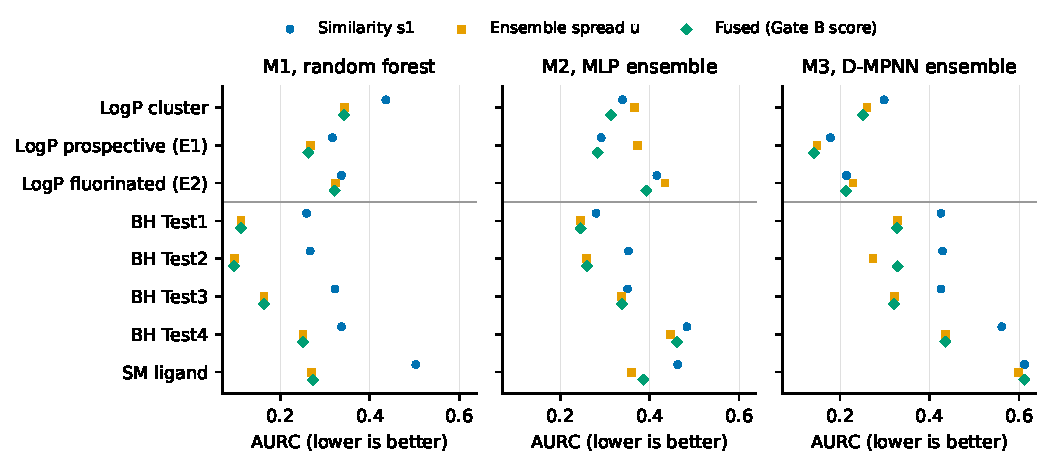
\includegraphics[width=\linewidth]{figures/fig7_signals_by_learner.pdf}
\caption{AURC of the selective error rate for each score on every held-out test, by learner (fusion fitted on $C_h$; mean over five seeds; lower is better). The horizontal line separates the logP tests (D1) from the reaction tests (D3). AURC levels also reflect each learner's ungated error rate, so the comparison is between the scores within a panel. M3 was added by protocol amendment 2.0.}
\label{fig:learners}
\end{figure}

The graph-network ensemble (M3) was the most accurate of the three learners on every logP test and the least accurate on every reaction test (Table~S11). On the held-out logP clusters its RMSE was 0.72 log units, against 0.90 for M1 and 0.84 for M2. On the fluorinated set E2 it was 0.44, against 0.61 and 0.70, and on the sp\textsuperscript{3} C--F compounds alone its $R^2$ was 0.31, where M1 and M2 were below zero. On the held-out BH tests its RMSE was 14.1--21.2 percentage points, against 10.8--17.8 for M1, and on the SM ligand test 22.3, against 20.1. Of its 175 members, 103 reached their lowest validation loss in the last three of the 50 epochs, so the default training budget may have limited M3, above all on the small reaction fit sets (about 1,640 and 2,690 reactions).

Its signals behaved like those of M1, not M2 (Figure~\ref{fig:learners}). Spread ranked errors better than similarity on seven of the eight held-out tests; the exception was E2, where similarity was slightly better (AURC 0.214 against 0.229). The fused score improved on the better single signal by 3.4\% and 4.3\% on the logP cluster and E1 tests and by less than 1\% on four others, and it was worse on the SM test (by 2.0\%) and on BH Test2 (by 20.1\%), where the scorer fitted on the held-out calibration fold transferred poorly. H3 therefore fails for M3 as well. Across the three learners, fusion never reached the 10\% that H3 requires, and which single signal ranked errors better depended on the learner and the task.

M3 met the H1 criterion on seven tests, including E2, where M1 had not (difference $-0.061$, 95\% interval $[-0.120, -0.010]$), and missed it on the SM test ($-0.004$, $[-0.028, +0.016]$). Its gates abstained more often than M1's. At $t = 0.8$, the $C_h$ pipeline accepted queries only on the three logP tests and BH Test2, at coverages of 0.02--0.11, and the $C_r$ pipeline accepted almost no reactions: the 50 highest-scoring calibration points were seldom accurate enough to pass the binomial test (Tables~S9, S10, S13 and S14). H2 fails because the random-fold pipeline never missed its target by more than 0.05: on logP it came within 0.05 of it, and on reactions it abstained. Intervals calibrated on $C_r$ covered at least 0.85 of the queries on seven held-out tests and 0.82 on BH Test4. On logP they did so at widths similar to M1's, about 2 log units; on reactions only because they were wide, 59--88 percentage points on average on the BH tests against 23--28 for M1 (exploratory, \texttt{results/amendment2}). On BH Test4 the $C_h$ gate accepted nothing, so recovery could not be checked there, and H4 fails, as note 1.1 of the protocol requires.

\subsection{Limitations}
\label{sec:limits}

The study is retrospective: every split was drawn from existing data, and no prediction was tested by new measurement. The reaction datasets come from two high-throughput campaigns with narrow chemistry, so a held-out additive or ligand is a modest shift. Their results say little about yields on diverse substrates. E2 is small (183 compounds), and its narrow logP range makes $R^2$ sensitive to modest absolute error; negative $R^2$ does not imply absent rank association. We used two fingerprint learners and, by a later amendment, one graph network with default settings; other architectures, tuned models and other uncertainty estimates may rank errors differently. The graph network was added after version 1 had been scored, so its motivation is post hoc, although its settings and criteria were fixed before it was run; it was trained for Chemprop's default 50 epochs, and most members were still improving at the end. The gate's threshold test starts at 50 calibration points, which makes it abstain whenever the most confident queries are not almost all correct; other starting points or a Bonferroni correction over the grid would behave differently. The SM test touched only seven of the twelve ligands across five seeds, and per-ligand results vary widely. The correctness thresholds of 0.5 log units and 10 percentage points are choices for illustration; a real context of use would set its own. The pooled cards describe the observed prediction--seed mixture, not a population of independent predictions. Neither the gate nor the interval implementation has an established finite-sample guarantee here. A future guarantee study would need independently fixed threshold candidates and order, independent calibration data, applicable multiple-testing control, fit/design-derived normalization, and mathematical and implementation review before new analyses. Chemistry-held-out calibration and test folds need not be exchangeable with each other. This unreviewed preprint does not validate a clinical system or establish FDA qualification. Finally, a shift that leaves the inputs looking familiar while changing the outcome, such as a change of assay protocol, is invisible to any input-based signal.

\section{Conclusions}

The tested pipelines often reduced accepted-set error at the cost of acceptance coverage, but all four complete pre-specified success criteria failed for the primary model. On seven of eight held-out tests, the fused score reduced error at 30\% coverage under the original query-bootstrap criterion; on the fluorinated hold-out it did not. At target precision 0.8, the chemistry-held-out pipeline reached higher descriptive precision than the random-fold pipeline on three BH tests, at lower coverage, while both missed the target on Test4. This compares complete pipelines: scorer fitting, threshold selection and calibration sizes change together, so the effect cannot be attributed to threshold calibration alone or ranked against signal choice. For the random forest, fusion added little to ensemble spread. The exploratory held-out interval-calibration rule often increased empirical coverage at the cost of width, without establishing conformal validity under shift or after gate selection. The neural ensemble ranked errors on all eight tests under the original criterion but its held-out pipeline abstained on all of them. A graph network, added by amendment, was the most accurate learner on logP and the least accurate on yields, but it did not change the outcome: spread ranked errors better than similarity on most tests, fusion added less than 10\%, and all four hypotheses failed again. These results support a bounded empirical contribution: evaluate complete abstention pipelines on chemistry-held-out tests, report achieved precision together with counts and coverage, and test a separately designed guarantee procedure in future work.

\section*{Supporting Information}
Tables S1--S3 (results of the MLP ensemble M2), Table S4 (operating-limits card of M1 at $t = 0.9$), the original analysis plan with amendment 2.0, revision limitations, Tables S5--S10 (per-seed Gate~B precision, correct/accepted counts and coverage for both pipelines and targets, for M1, M2 and M3), and Tables S11--S14 (results of the graph-network ensemble M3).

\section*{Data and code availability}
All data are public (SangsterLogP, CC BY 4.0;\cite{sangsterzenodo} the Buchwald--Hartwig, Suzuki--Miyaura and fluorinated-amide data under the MIT licence of their repositories). The code, the analysis plan, the split definitions, all per-query predictions and the scripts that regenerate every figure and table are available at \url{https://github.com/blackthorn-ai/accept-or-abstain} under the MIT licence.

\section*{Author contributions}
O.G.: conceptualization, methodology, software, formal analysis, interpretation, writing, review, and editing.

\section*{Competing interests}
O.G. is the director and owner of Blackthorn AI Ltd., which provides machine-learning services to life-sciences companies, including work on model reliability. No client data, code or results were used in this work.

\section*{Funding}
This work received no specific funding.

\bibliographystyle{unsrtnat}
\bibliography{references}

\end{document}
